\def\difficulty{3}
\sujet{Image Restoration: deconvolution}
\index{Restoration!Deconvolution}

\begin{note}This tutorial aims to study and test different image restoration methods for blurred and noisy images. Altough the different software tools contain functions for each filter 
the objective is to exhaustively code these methods to fully understand their principles. The reader can refer to \cite{Sage2017} for more informations on the algorithms.

Some of the images are based on observations made with the NASA/ESA Hubble Space Telescope, and obtained from the Hubble Legacy Archive, which is a collaboration between the Space Telescope Science Institute (STScI/NASA), the Space Telescope European Coordinating Facility (ST-ECF/ESA) and the Canadian Astronomy Data Centre (CADC/NRC/CSA). You may access to these resources at https://hla.stsci.edu/
\end{note}

% \begin{mcomment}
% (for example \minline{deconvwnr} or \minline{deconvlucy} for matlab), 
% \end{mcomment}

\noindent The different processes will be applied on the following images.
% https://cral.univ-lyon1.fr/labo/perso/eric.thiebaut/?Teaching

\section{Damage modeling}
\begin{figure}[!h]\caption{Images that can be used for testing the different restoration algorithms. Intensity levels are represented in false colors.}%
\begin{center}
	\vspace*{5pt}
\subfloat[Jupiter, from Hubble Space Telescope, \newline ads/Sa.HST\#ic3g01qlq.]{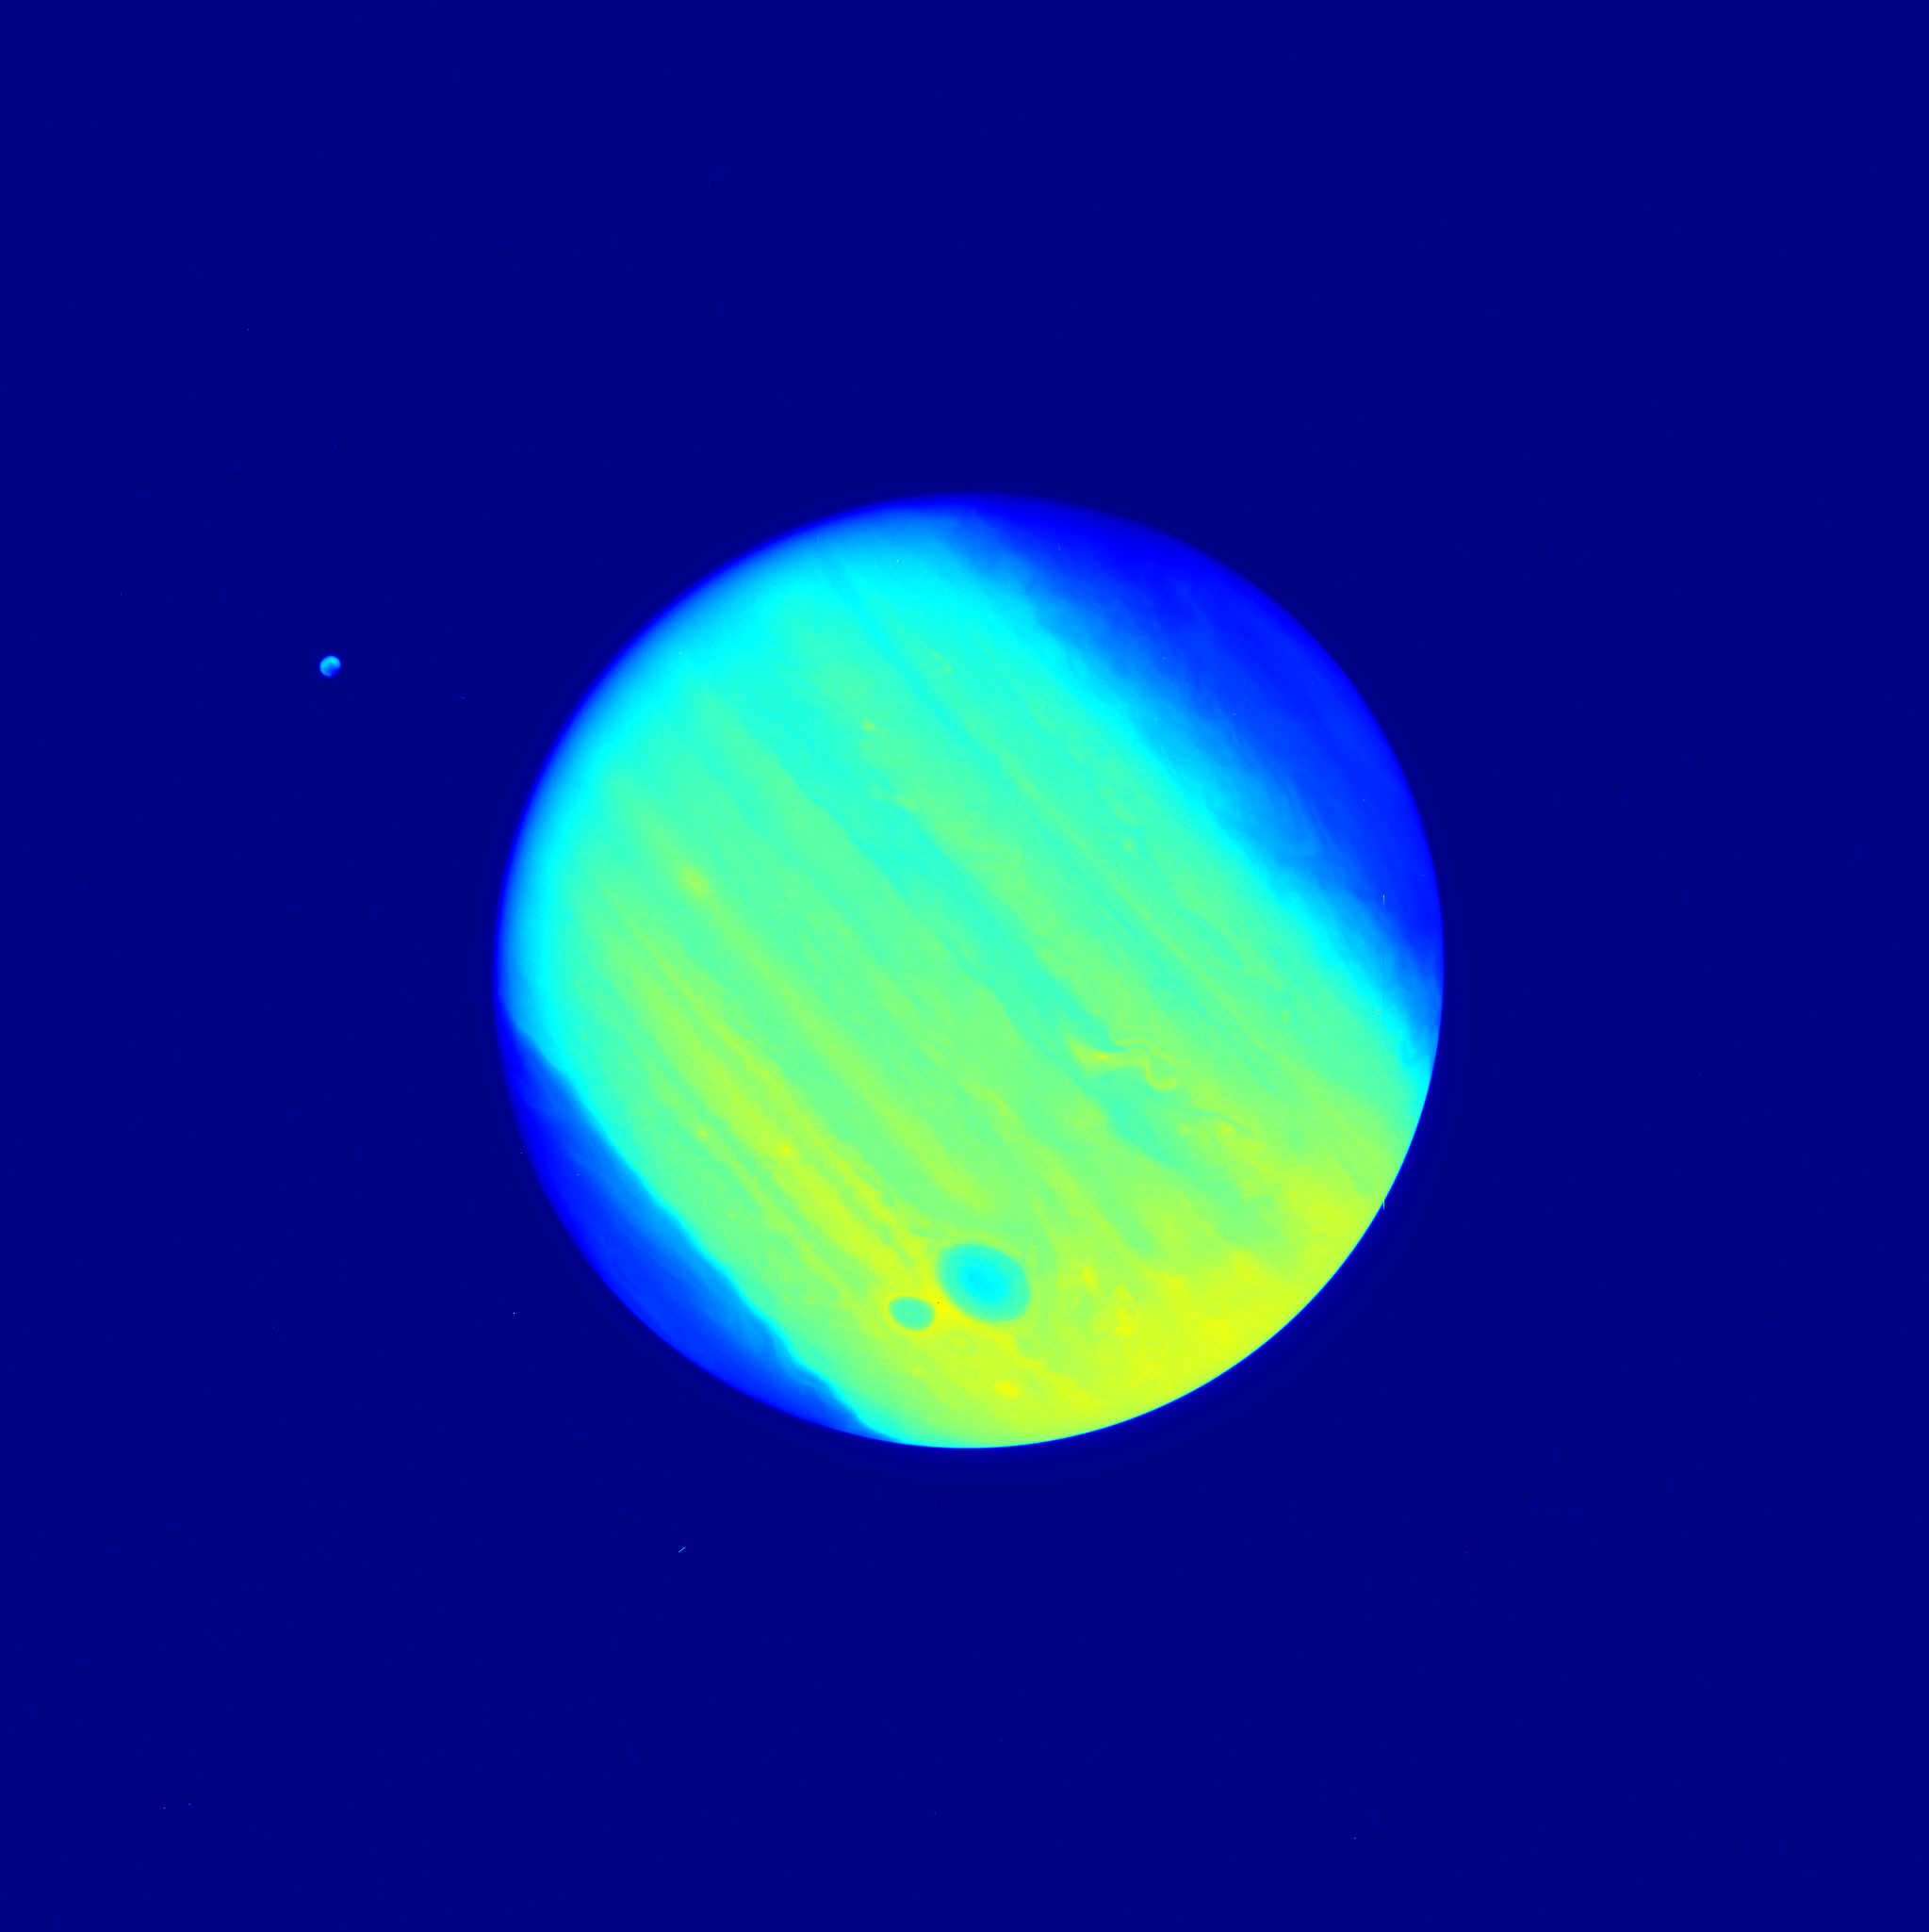
\includegraphics[width=6.5cm]{ic3g01qlq_flt.png}}
\hspace{1cm}
\subfloat[PSF for Jupiter image]{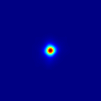
\includegraphics[width=3cm]{ic3g01qlq_psf.png}}

\subfloat[Saturn, HST.]{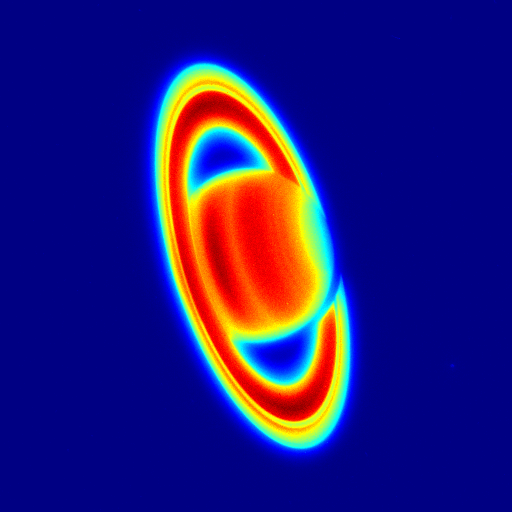
\includegraphics[width=6.5cm]{saturn.png}}
\hspace{1cm}
\subfloat[PSF for Saturn image]{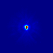
\includegraphics[width=3cm]{saturn_psf.png}}
\vspace*{-10pt}
\end{center}
\end{figure}

A damage process can be modeled by both a damage function $D$ and an additive noise $n$, acting on an input image $f$ for producing the damaged image $g$.
\begin{eqnarray}
g=D(f)+n
\end{eqnarray}
Knowing $g$, the objective of restoration is to get an estimate $\hat{f}$ (the restored image) of the original image $f$. If $D$ is a linear process, spatially invariant, then the equation can be simplified as:
\begin{eqnarray}
g=h*f+n \label{eq:damage}
\end{eqnarray}
where $h$ is the spatial representation of the damage function (called the Point Spread Function - PSF), and $*$ denotes the convolution operation.
In general, the more knowledge you have about the function $H$ and the noise $n$, the closer $\hat{f}$ is to $f$.\index{Point Spread Function}

This equation can be written in the frequency domain:\index{Fourier Transform}
\begin{eqnarray}
G=H.F+N
\end{eqnarray}
where the letters in uppercase are the Fourier transforms of the corresponding terms in the eq. \ref{eq:damage}.

	\begin{figure}[htbp]
	 \centering\caption{Chessboard image.}%
	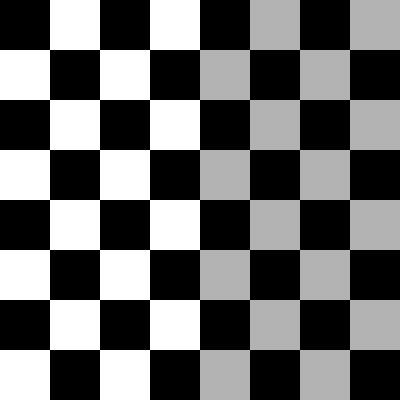
\includegraphics[height=3.25cm]{chessboard}%
	\end{figure}
	
\begin{qbox}
\begin{itemize}
	\item Generate the 'chessboard' image.
	\item Generate a PSF corresponding to a blur (motion or isotropic).
	\item Create a damaged image (a circular option is used, because the FFT implies that functions are periodical) and add a Gaussian noise.
	\item Visualize the different images. 
\end{itemize}
\end{qbox}

\begin{mcomment}
\begin{mremark}
 \matlabregistered{} has a \minline{checkerboard} function for the 'chessboard' image. The \minline{fspecial} function generates a convolution matrix.
\end{mremark}
\end{mcomment}


\section{Simple case: no noise}\index{Fourier Transform!Inverse}
The objective is now to restore the damaged image.

For the first steps, no noise will be added. The degradation functions is $g=h*f$. Knowing $H$ (Fourier Transform of the psf $h$) and ignoring the noise in the damage model, a simple estimate of the initial image can be done by the inverse filtering:
\begin{eqnarray}
f=FT^{-1}\left(\frac{G}{H}\right)
\end{eqnarray}
where $FT^{-1}$ denotes the inverse Fourier transform.

\begin{qbox}
 \begin{itemize}
  \item Try the inverse filter in the Fourier space. Why is this filter not working?
  \item Try to prevent division by 0, with $f=FT^{-1}\left(\frac{G}{H+\alpha}\right)$, $\alpha$ being a small constant value (e.g. $\alpha=0.1$).
 \end{itemize}
\end{qbox}

\section{Wiener filter}
\index{Restoration!Wiener filter}
The Wiener filter is an optimal filter that minimizes the following error:
\begin{eqnarray*}
e^2=E\{(f-\hat{f})^2\}
\end{eqnarray*}
where $E$ denotes the expected (mean) value, $f$ is the original image and $\hat{f}$ is the restored image.

The solution to this expression, within the frequency domain, is given by:
\begin{eqnarray*}
\hat{F}=\underbrace{\left(\frac{1}{H}\frac{|H|^2}{|H|^2+R}\right)}_{H_w}G
\end{eqnarray*}

The value of $R$ can be arbitrarily fixed. Another way is to define $R=S_n/S_f$, where $S_n$ and $S_f$ denote the power spectrum of the noise $n$ and the original image $f$, i.e. $|N|^2$ and $|F|^2$ (matrices), respectively. This ratio can be defined globally (as the constant) or locally (i.e. it is computed for each pixel). If the ratio $S_n/S_f$ (function) is non null, it can be passed to the Wiener filtering process.

\subsection{Simple case: no noise}

In the noiseless case, the Wiener filter reduces to the inverse filter:
$$
{H_w}=\left\{
\begin{array}{ll}
\displaystyle\frac{1}{H(u,v)}&\text{ if } |H(u,v)|\neq 0\\
0 & \text{ otherwise}
\end{array}
\right.
$$
\begin{qbox}
Try a Wiener filter for the noiseless case.
\end{qbox}

\subsection{Noisy images}

Generally, the ratio $S_n/S_f$ used in the Wiener filter is replaced by a constant value equal to the ratio of the mean power spectrum:
\begin{eqnarray}
R=\frac{\displaystyle\frac{1}{PQ}. \sum_u\sum_v S_n(u,v)}{\displaystyle\frac{1}{PQ}.\sum_u\sum_v S_f(u,v)}
\end{eqnarray}
where $PQ$ denotes the matrix size (the number of elements).

\begin{mcomment}
 \begin{mremark}
   see \minline{numel} function.
 \end{mremark}
\end{mcomment}

\begin{qbox}
\begin{enumerate}
	\item Calculate the constant ratio $R$ and code the Wiener filter .
	\item Test the different algorithms on the image 'brain' damaged by a blur and an additive noise.
\end{enumerate}
\end{qbox}


\section{Iterative filters for noisy images}

\subsection{Van Cittert iterative filter}\index{Restoration!Van Cittert filter}
The VanCittert iterative filter is based on the following iterative relation :
$$f_{k+1}=f_k+\beta(g-h*f_k)$$
with $f_0=g$, the damaged image.

\begin{qbox}
Code and test on different cases a function that performs the VanCittert restoration filter.  
\end{qbox}

It should have the following prototype:
\begin{matlab}
function [ fr ] = vca( g, psf, n_iter)
% Van Cittert iteration algorithm for deconvolution
%
% g: degraded image
% psf: point spread function
% n_iter: number of iterations
\end{matlab}

\begin{python}
def vca(g, psf, n_iter, beta=.01):
    """
    Van Cittert iterative filter
    g: noisy image
    psf: point spread function
    n_iter: number of iterations
    beta: Jansson parameter
    """
\end{python}


\subsection{Lucy-Richardson filtering}\index{Restoration!Lucy-Richardson filter}
We are now going to use the nonlinear restoration filtering of Lucy-Richard\-son that is based on a maximum likelihood formulation in which the image is modeled by Poisson statistics. This optimization leads to the solution if the following iterative equation converges:
\begin{eqnarray}
{f}_{k+1}(x,y)={f}_{k}(x,y)\cdot \left(h(-x,-y)*\frac{g(x,y)}{h(x,y)*{f}_k(x,y)}\right)
\end{eqnarray}

\begin{qbox}
Code and test your own function for the Lucy-Richardson filtering process. It should have the same prototype as the VanCittert function. Remember that $\cdot$ is the classical multiplication (point to point) and that $*$ is the convolution operation. You then have the choice to make a direct call to the convolution function, or to perform this operation in the Fourier space.
\end{qbox}

\section{Blind deconvolution: restoration with no a priori}\index{Restoration!Blind deconvolution}
If the PSF is unknown, one of the main difficulties in image restoration is to get an accurate estimate of this PSF in order to use it in the deconvolution algorithms. These methods are called blind deconvolution methods. Generally, the PSF is estimated in an iterative way from an initial PSF.

\begin{qbox}
\begin{enumerate}
	\item Generate a damaged image of 'chessboard' with a Gaussian blur and an additive Gaussian noise.
	\item Restore from a blind deconvolution the damaged image and compare the results with the previous ones.
\end{enumerate}

\end{qbox}
\begin{mcomment}
\begin{mremark}
 Use the function \minline{deconvblind}.
\end{mremark}
\end{mcomment}

\begin{phelp}
 Use the function \pinline{skimage.restoration.unsupervised_wiener} for example.
\end{phelp}


\section{Astronomy images}

A classical file format used in astronomy is the FITS format. 

\begin{mcomment}
\begin{mremark}
The \textbf{FITS} files can be read using the function \minline{fitsread}. For example, the following commands will read an image and its PSF.

\begin{matlab}
% 1st example
saturn = fitsread('saturn.fits');
psf = fitsread('saturn_psf.fits');

% 2nd example
jupiter = fitsread('ic3g01qlq_flt.fits', 'image', 1);
psf = fitsread('PSFSTD_WFC3UV_F275W.fits');
jupiter_psf = p(:,:,1); % select 1st psf only
\end{matlab}

\end{mremark}
\end{mcomment}

\begin{pcomment}
\begin{premark}
 With python, fits images can be manipulated with the \pinline{astropy} module. You can use the following code to display an image.
\end{premark}
 \begin{python}
hdu_list = fits.open('ic3g01qlq_drz.fits');
image = hdu_list[1].data;
image = np.nan_to_num(image);
plt.imshow(image, cmap='gray')
plt.show()
 \end{python}
\end{pcomment}
